\chapter*{Project 1: DNA Analysis}
\addcontentsline{toc}{chapter}{Project 1: DNA Analysis}
\setcounter{chapter}{7}
\setcounter{section}{0}


\section{Introduction}
You have recently been employed by Rhonda Labs, a leading research institute working to uncover the secrets of rare genetic diseases. Your first task is to write a program that analyzes DNA from various species and individuals, compares their similarities, and performs analyses on the given sequences.


Before you dive into the project, let's review a bit of biology to help you understand what you will be working with. DNA, or deoxyribonucleic acid, is the molecule that carries genetic information in almost all living organisms. It acts like a set of instructions that tells cells how to function, grow, and reproduce.

DNA is made up of four chemical bases:
\begin{itemize}[left=1cm]
    \item Adenine (A)
    \item Cytosine (C)
    \item Guanine (G)
    \item Thymine (T)
\end{itemize}

\begin{figure}[htp]
    \centering
    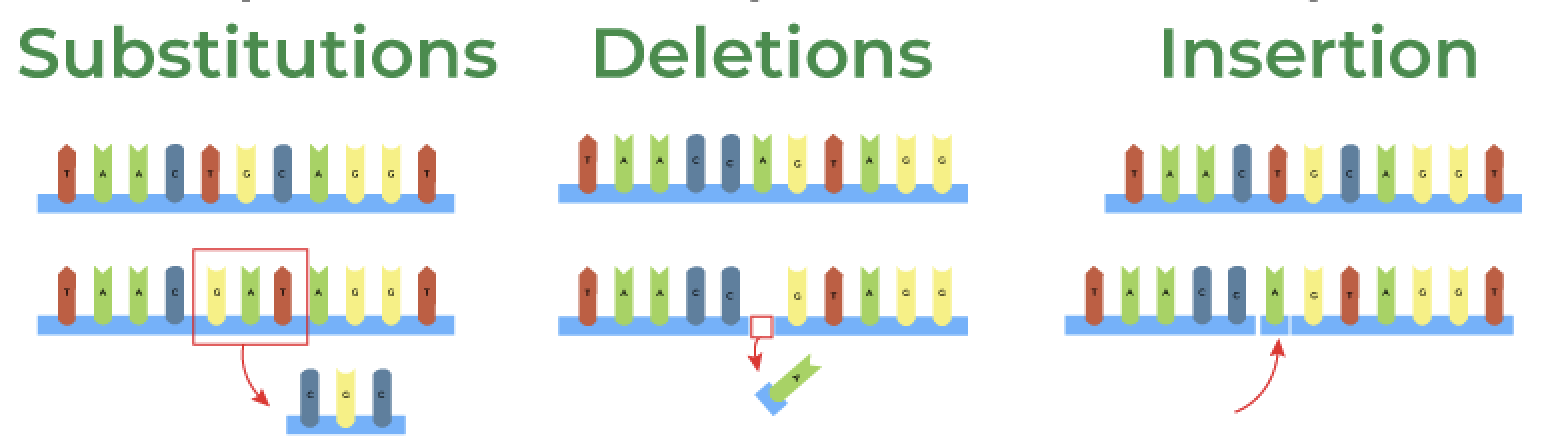
\includegraphics[width=12cm]{images/project1/newMutationsImg.png}
    \caption{Types of DNA mutations}
    \label{fig:galaxy}
\end{figure}

These bases pair together (A with T, C with G) to form the DNA double helix, which is the the overall structure of DNA. A DNA strand is made up of a sequence of these base pairs. Every organism has its own unique DNA sequence, though many organisms share similarities, especially related species. Sometimes, DNA sequences can change, leading to mutations, such as:

\begin{itemize}[left=1cm]
    \item Substitutions (one base is swapped for another)
    \item Insertions (extra bases are added)
    \item Deletions (bases are removed)
\end{itemize}

For this task, the steps are outlined and divided into individual questions. By the end of the project, you will have developed a cohesive program that a user can interact with by inputting their DNA sequences. Below is a breakdown of the steps: 

\begin{enumerate}[left=1cm]
    \item Check whether your DNA strands are composed of valid bases
    \item Develop functions to compare DNA strands and assess their similarity
    \item Develop a function that compares two DNA sequences and identifies all types of mutations between them
    \item Transcribe DNA to RNA and compute the reverse complement of a DNA strand
    \item Find open reading frames within a DNA strand
    \item Final step:  make it more accessible and user-friendly!
    
\end{enumerate}


\section{Assignment}

\textbf{Warning: You are not allowed to use global variables for this project.}

All function names, return types, and parameters must precisely match those shown. You may not use pass by reference or otherwise modify the function prototypes. You are welcome to create additional functions that may help streamline your code. You must well comment your code, and follow good formatting practices. You should create assert statements for each function to test your code in VS Code before moving to CodeRunner.

\subsection{Question 1: \texttt{isValidBase()}}
One of the first steps when working with DNA sequences is to check whether the data is valid or corrupted. You must ensure the sequences you are working with consist only of valid DNA bases: A, C, G, and T. You will write a function, \texttt{isValidBase()}, that checks if a character is a valid DNA base.

\begin{longtable}{|p{1.7in}|p{4.0in}|}
    \hline
    \textbf{Function:} \texttt{isValidBase(char)}
        & 
        \mintinline{c++}{bool isValidBase(char base)}
        \\ \hline
    \textbf{Purpose:} 
        & 
        The function will determine whether a given character is a valid DNA base. The function should not print anything. 
        \\ \hline
    
    \textbf{Parameters:} 
        & 
        \textbf{char} \texttt{base} - The character to validate. 
        \\ \hline
    
    \textbf{Return Value:} 
        & 
        The function should return true if the character is a valid base (A, C, G, or T) and false otherwise. 
        \\ \hline
    \textbf{Error handling/ Boundary conditions:}
        &
        - The function should be case-sensitive, e.g., `A' is a valid base, but `a' is not. \newline
        - \textbf{Note:} True is represented by 1 and false by 0 when you \mintinline{c++}{cout} boolean variables.
        \\ \hline
\end{longtable}

\textbf{For Question 1, develop and validate your solution in VS Code. Once you are happy with your solution, go to coderunner on Canvas and paste only the \texttt{isValidBase()} to the answer box!} 

\begin{sampleProject}
    \hspace{0pt}
    \begin{longtable}{|p{2.0in}|p{2.0in}|}
        \hline
        \textbf{Function call}
            & 
            \textbf{Expected return value}
            \\ \hline
        
        isValidBase('A')
            & 
            true
            \\ \hline
        
        isValidBase('X')
            & 
            false
            \\ \hline
        
        isValidBase('a')
            & 
            false
            \\ \hline

        isValidBase('T')
            & 
            true
            \\ \hline
    \end{longtable}

\end{sampleProject}

\subsection{Question 2: \texttt{isValidStrand()}}

Next, write the \texttt{isValidStrand()} function that checks if a string contains only valid DNA bases.

\begin{longtable}{|p{1.7in}|p{4.0in}|}
    \hline
    \textbf{Function:} \texttt{isValidStrand(string)}
        & 
        \mintinline{c++}{bool isValidStrand(string strand)} 
        \\ \hline
    
    \textbf{Purpose:} 
        & 
        The function will determine whether a given string consists only of valid DNA bases. The function should not print anything.
        \\ \hline
    
    \textbf{Parameters:} 
        & 
        \textbf{string} \texttt{strand} - The DNA strand to validate. 
        \\ \hline
    
    \textbf{Return Value:} 
        & 
        The function should return true if the string is a valid DNA strand and false otherwise.
        \\ \hline
    \textbf{Error handling/ Boundary conditions:}
        &
        - The input string is only considered valid if it consists only of A, C, T, and G bases. \newline
        - If the string is empty, then it should not be considered a valid DNA strand, and your function should return false. \newline
        - \textbf{Hint:} The function should make use of your \texttt{isValidBase} function.
        \\ \hline
\end{longtable}

\textbf{For Question 2, develop and validate your solution in VS Code. Once you are happy with your solution, go to coderunner on Canvas and paste the \texttt{isValidBase()} and \texttt{isValidStrand()} to the answer box!} 

\begin{sampleProject}
    \hspace{0pt}
    \begin{longtable}{|p{2.0in}|p{2.0in}|}
        \hline
        \textbf{Function call}
            & 
            \textbf{Expected return value}
            \\ \hline
        
        isValidStrand("ATGCTTCAA")
            & 
            true
            \\ \hline
        
        isValidStrand("CTTZ")
            & 
            false
            \\ \hline
        
        isValidStrand("")
            & 
            false
            \\ \hline

        isValidStrand("ATCG")
            & 
            true
            \\ \hline
    \end{longtable}
\end{sampleProject}


\subsection{Question 3: \texttt{strandSimilarity()}}

Comparing DNA sequences allows researchers to identify similarities and differences that may be significant in understanding genetic relationships or disease mechanisms. In this step, you'll develop functions to compare DNA strands and assess their similarity.

For two DNA strands of equal length, the similarity score is calculated based on the number of matching bases at corresponding positions using the following formula:

\[
\text{Similarity} = \frac{\text{total matches}}{\text{total positions}}
\]

\textbf{Example:}
Let's compare the following two DNA strands:

\begin{table}[htbp]
    \centering
    \begin{tabular}{|c|c|c|}
    \hline
    \textbf{Position} & \textbf{Strand 1} & \textbf{Strand 2} \\
    \hline
    1 & G & G \\
    2 & A & T \\
    3 & T & T \\
    4 & C & C \\
    5 & A & A \\
    6 & G & A \\
    \hline
    \end{tabular}
    \caption{Positions of two DNA strands}
\end{table}

The total number of matches is 4 out of 6 positions, resulting in a similarity score of \( \frac{4}{6} = 0.667 \).

\hspace{0pt}

The function \mintinline{c++}{strandSimilarity()} compares two strands position by position, counting the number of positions where the bases are identical. This provides a direct measure of how similar the two sequences are.

\begin{longtable}{|p{1.7in}|p{4.0in}|}
    \hline
    \textbf{Function:} \texttt{strandSimilarity(string, string)}
        & 
        \mintinline{c++}{double strandSimilarity(string strand1, string strand2)} 
        \\ \hline
    
    \textbf{Purpose:} 
        & 
        The function will find the similarity between two DNA strands. The function should not print anything.
        \\ \hline
    
    \textbf{Parameters:} 
        & 
        \textbf{string} \texttt{strand1} - The first DNA strand to compare. \newline
        \textbf{string} \texttt{strand2} - The second DNA strand to compare. 
        \\ \hline
    
    \textbf{Return Value:} 
        & 
        The function should return the similarity score between the two strands. 
        \\ \hline
    \textbf{Error handling/ Boundary Condition:}
        &
        - The parameters should be two strings of equal length. If they are not equal in length, your function should return 0. \newline
        - You may assume that the input to \mintinline{c++}{strandSimilarity()} will always be a valid strand, i.e., you do not have to account for arbitrary strings.
    \\ \hline
\end{longtable}

\textbf{For Question 3, develop and validate your solution in VS Code. Once you are happy with your solution, go to coderunner on Canvas and paste the \texttt{strandSimilarity()} and any helper function(s) you used to the answer box!} 

\begin{sampleProject}
    \hspace{0pt}
    \begin{longtable}{|p{3.0in}|p{2.5in}|}
        \hline
        \textbf{Function call}
            & 
            \textbf{Expected return value}
            \\ \hline
        
        strandSimilarity("AGGT" , "CTGA")
            & 
            0.25
            \\ \hline
        
        strandSimilarity("CCTT" , "CCTT")
            & 
            1
            \\ \hline
        
        strandSimilarity("ATG" , "AAATTT")
            & 
            0
            \\ \hline

        strandSimilarity("CTGTAGAGCT" , "TAGCTACCAT")
            & 
            0.2
            \\ \hline
    \end{longtable}
\end{sampleProject}

\hspace{2pt}

\subsection{Question 4: \texttt{bestStrandMatch()}}

In \mintinline{c++}{bestStrandMatch()}, the strands can be different lengths, therefore, you'll want to compare overlapping sections and calculate similarity scores at each position, and to do that you'll slide the shorter strand along the longer strand. The maximum score across all positions indicates the best alignment between the two strands.

\begin{longtable}{|p{1.7in}|p{4.0in}|}
    \hline
    \textbf{Function:} \texttt{bestStrandMatch(string, string)}
        & 
        \mintinline{c++}{int bestStrandMatch(string input_strand, }
        \mintinline{c++}{string target_strand)}

        \\ \hline
    
    \textbf{Purpose:} 
        & 
        The function will find the best similarity between two DNA strands. The function should print out the best similarity score.
        \\ \hline
    
    \textbf{Parameters:} 
        & 
        \textbf{string} \texttt{input\_strand} - The input DNA strand to be checked against the target\_strand (length greater than or equal to the target strand) \newline
\textbf{string} \texttt{target\_strand} - The target DNA strand.\\ \hline
    
    \textbf{Return Value:} 
        & 
        If the parameters are valid, returns an \mintinline{c++}{int} representing the starting index of the substring in the input strand where the best alignment with target strand occurs.
        
        \\ \hline
    \textbf{Error handling/ Boundary conditions:} 
        &
        - If the input strand is shorter than the target strand, the function returns -1 as the alignment index and prints out "Best similarity score: 0.0". \newline
- This function should make use of the \mintinline{c++}{strandSimilarity()} function. \newline
- You may assume that the input to \texttt{bestStrandMatch()} will always be a valid DNA sequence, i.e., you do not have to account for arbitrary strings.\\ \hline
\end{longtable}

\textbf{For Question 4, develop and validate your solution in VS Code. Once you are happy with your solution, go to coderunner on Canvas and paste the \texttt{bestStrandMatch()} and any helper function(s) you used to the answer box!}  

\begin{figure}[htp]
    \centering
    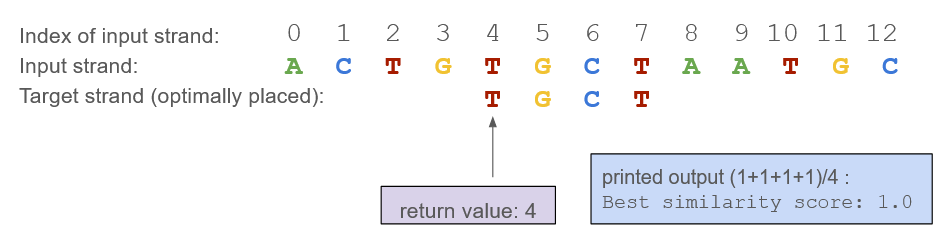
\includegraphics[width=12cm]{images/project1/BestSimilarity.png}
    \caption{An illustration of bestStrandMatch() between two example strands}
    \label{fig:galaxy}
\end{figure}

\begin{sampleProject}
    \hspace{0pt}
    \begin{longtable}{|p{1.8in}|p{1.8in}|p{1.8in}|}
        \hline
        \textbf{Function call}
            & 
            \textbf{Expected return value}
            & 
            \textbf{Expected printed value}
            \\ \hline
        
        \texttt{bestStrandMatch("GATCAGT", "TCA")}
            & 
            2
            &
            \texttt{Best similarity score: 1.0}
            \\ \hline
        
        \texttt{bestStrandMatch("AACCTGAC", "ACT")}
            & 
            1
            &
            \texttt{Best similarity score: 0.666667}
            \\ \hline
        
        \texttt{bestStrandMatch("CTG", "CCCC")}
            & 
            -1
            &
            \texttt{Best similarity score: 0.0}
            \\ \hline

        \texttt{bestStrandMatch("ATCGTA", "TTCGAT")}
            & 
            0
            &
            \texttt{Best similarity score: 0.5}
            \\ \hline
    \end{longtable}
\end{sampleProject}


\subsection{Question 5: Mutation Detection}

Now, you want to be able to make deeper observations between DNA sequences. To do this, you will create a function that compares two DNA sequences and identifies all types of mutations between them. The function should align the sequences based on the best possible match and then process the sequences character by character, printing out mutations as they are detected.

Your function should be able to identify the following mutations:
\begin{itemize}[left=1cm]
    \item Substitution: When bases at the same position differ
    \item Insertion: When an extra base is present in the target strand
    \item Deletion: When a base from the input strand is missing in the target strand
\end{itemize}

The function should determine the longest of the two strands and use the \mintinline{c++}{bestStrandMatch()} function to optimally align them. Upon alignment, the function should print out the best alignment index. After alignment, it should compare the sequences character by character to identify mutations. It detects substitutions when bases at the same aligned position differ, deletions when extra bases are present in the input strand but not in the target strand, and insertions when bases are present in the target strand but missing from the input strand.


\begin{longtable}{|p{1.7in}|p{4.0in}|}
    \hline
    \textbf{Function:} \newline identifyMutations(string, string)
        & 
        \mintinline{c++}{void identifyMutations(string input_strand, }
        \mintinline{c++}{string target_strand)} 
        \\ \hline
    
    \textbf{Purpose:} 
        & 
        The function compares two DNA sequences to identify all types of mutations between them. It aligns the sequences based on the best possible match and processes them character by character, printing out any mutations as they are detected.
        \\ \hline
    
    \textbf{Parameters:} 
        & 
        \textbf{string} \texttt{input\_strand} - The input strand to be checked against the target
        
        \textbf{string} \texttt{target\_strand} - The target strand
        \\ \hline
    
    \textbf{Return Value:} 
        & 
        N/A
        \\ \hline
    \textbf{Error handling/ Boundary conditions:} 
        &
        -You may assume that the input and target strands are both valid DNA strands.
        
        - If no mutations are found, the function outputs ``No mutations found."

       
    \\ \hline
\end{longtable}

\textbf{For Question 5, develop and validate your solution in VS Code. Once you are happy with your solution, go to coderunner on Canvas and paste \texttt{identifyMutations()} and any helper function(s) to the answer box!} 

\begin{figure}[htp]
    \centering
    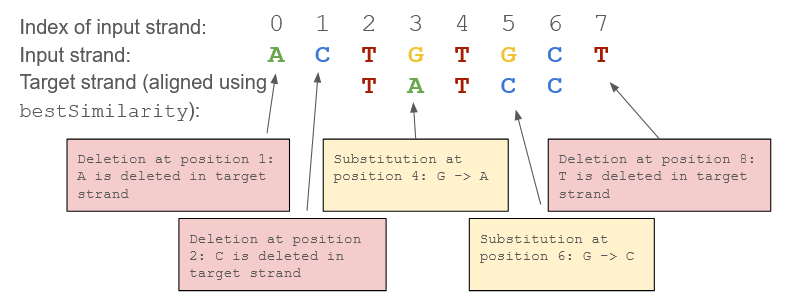
\includegraphics[width=12cm]{images/project1/mutationDetection.png}
    \caption{An illustration of identifyMutation() between two example strands}
    \label{fig:galaxy}
\end{figure}

\begin{sampleProject}

\textbf{Note: "Best Similarity Score:..." print line should come from your \mintinline{c++}{bestStrandMatch()} function.}
    \hspace{0pt}
    \begin{longtable}{|p{2.6in}|p{2.5in}|}
        \hline
        \textbf{Function call}
            & 
            \textbf{Expected printed value}
            \\ \hline
        
        identifyMutations("GGG", "TAGGGTA")
            & 
            Best similarity score: 1
            
            Best alignment index: 2

            Insertion at position 1: T is inserted in target strand

            Insertion at position 2: A is inserted in target strand

            Insertion at position 6: T is inserted in target strand
            
            Insertion at position 7: A is inserted in target strand
            
            \\ \hline
        
        identifyMutations("AACCGG", "AACCGG")
            & 
            Best similarity score: 1
            
            Best alignment index: 0
            
            No mutations found.
            \\ \hline
        
        identifyMutations("TA", "TAGG")
            & 
            Best similarity score: 1
            
            Best alignment index: 0
            
            Insertion at position 3: G is inserted in target strand

            Insertion at position 4: G is inserted in target strand
            \\ \hline

        identifyMutations("TAGG", "TA")
            & 
            Best similarity score: 1
            
            Best alignment index: 0


            Deletion at position 3: G is deleted in target strand

            Deletion at position 4: G is deleted in target strand
            \\ \hline

        identifyMutations("AGTCACG", "AGCTACA")
            & 
            Best similarity score: 0.571429
            
            Best alignment index: 0
            
            Substitution at position 3: T -> C
            
            Substitution at position 4: C -> T
            
            Substitution at position 7: G -> A
            \\ \hline
    \end{longtable}
\end{sampleProject}

\subsection{Question 6: DNA Sequence Transformations}

In this part, you will simulate the transcription process by converting a DNA sequence into an RNA sequence. This involves replacing every occurrence of thymine (`T') with uracil (`U') in the DNA strand.

\begin{longtable}{|p{1.7in}|p{4.0in}|}
    \hline
    \textbf{Function:} \texttt{transcribeDNAtoRNA(string)}
        & 
        \mintinline{c++}{void transcribeDNAtoRNA(string strand)} 
        \\ \hline
    
    \textbf{Purpose:} 
        & 
        The function will transcribe a DNA sequence to RNA and print the RNA sequence to the console. The function will replace all occurrences of `T' with `U'.
        \\ \hline
    
    \textbf{Parameters:} 
        & 
        \textbf{string} \texttt{strand} - The DNA sequence to be transcribed.
        \\ \hline
    
    \textbf{Return Value:} 
        & 
        N/A
        \\ \hline
    \textbf{Error handling/ Boundary conditions:}
        &
        - You may assume that the input DNA strand is a valid DNA sequence.
        \\ \hline
\end{longtable}

\textbf{For Question 6, develop and validate your solution in VS Code. Once you are happy with your solution, go to coderunner on Canvas and paste \texttt{transcribeDNAtoRNA()} and any helper function(s) to the answer box!}  


\begin{sampleProject}
    \hspace{0pt}
    \begin{longtable}{|p{2.6in}|p{2.5in}|}
        \hline
        \textbf{Function call}
            & 
            \textbf{Expected printed value}
            \\ \hline
        
        transcribeDNAtoRNA("ATCGTACG")
            & 
            AUCGUACG
            \\ \hline
        
        transcribeDNAtoRNA("TTAA")
            & 
            UUAA
            \\ \hline
        
        transcribeDNAtoRNA("ACCG")
            & 
            ACCG
            \\ \hline

        transcribeDNAtoRNA("T")
            & 
            U
            \\ \hline
    \end{longtable}
\end{sampleProject}

\hspace{15pt}

\subsection{Question 7: Reverse Complement of a DNA Sequence}

In this part, you will write a function to compute the reverse complement of a DNA strand. The reverse complement is obtained by reversing the DNA sequence and then replacing each base with its complement:
\begin{itemize}[left=1cm]
    \item `A' is complemented by `T'
    \item `T' is complemented by `A'
    \item `C' is complemented by `G'
    \item `G' is complemented by `C'
\end{itemize}

\begin{longtable}{|p{1.7in}|p{4.0in}|}
    \hline
    \textbf{Function:} \texttt{reverseComplement(string)}
        & 
        \mintinline{c++}{void reverseComplement(string strand)} 
        \\ \hline
    
    \textbf{Purpose:} 
        & 
        The function will compute the \textbf{reverse} complement for a DNA sequence and print the result to the console.
        \\ \hline
    
    \textbf{Parameters:} 
        & 
        \textbf{string} \texttt{strand} - The DNA sequence for which the reverse complement will be computed.
        \\ \hline
    
    \textbf{Return Value:} 
        & 
        N/A
        \\ \hline
    \textbf{Error handling/ Boundary condition:}
        &
        You may assume that the input DNA strand is a valid DNA sequence.
    \\ \hline
\end{longtable}

\textbf{For Question 7, develop and validate your solution in VS Code. Once you are happy with your solution, go to coderunner on Canvas and paste the \texttt{reverseComplement()} and any helper function(s) you used to the answer box!} 

\begin{sampleProject}
    \hspace{0pt}
    \begin{longtable}{|p{2.6in}|p{2.5in}|}
        \hline
        \textbf{Function call}
            & 
            \textbf{Expected printed value}
            \\ \hline
        
        reverseComplement("ATCGTACG")
            & 
            CGTACGAT
            \\ \hline
        
        reverseComplement("AAACCC")
            & 
            GGGTTT
            \\ \hline
        
        reverseComplement("AGCT")
            & 
            AGCT
            \\ \hline

        reverseComplement("A")
            & 
            T
            \\ \hline
    \end{longtable}
\end{sampleProject}

\subsection{Question 8: Extracting Reading Frames}

%This should be updated so it is clear that ORFs cannot overlap. 

When working with DNA sequences, it is often necessary to focus on specific regions called open reading frames (ORF). These DNA regions are read in groups of three bases, called codons, which are later translated into amino acids during the process of protein synthesis. An ORF is a continuous sequence of DNA that begins with a start codon (ATG) and ends with a stop codon (TAA, TAG, or TGA).  

\hspace{0pt}

Your task is to identify valid protein-coding regions in a DNA sequence. A valid ORF starts with the ATG codon and ends with one of the stop codons (TAA, TAG, or TGA), with the number of bases between the start and stop codons being divisible by 3.


\begin{longtable}{|p{1.7in}|p{4.0in}|}
    \hline
    \textbf{Function:} \texttt{getCodingFrames(string)}
        & 
        \mintinline{c++}{void getCodingFrames(string strand)} 
        \\ \hline
    
    \textbf{Purpose:} 
        & 
        The function will print out complete reading frames.
        \\ \hline
    
    \textbf{Parameters:} 
        & 
        \textbf{string} \texttt{strand} - The DNA strand from which to extract reading frames.
        \\ \hline
    
    \textbf{Return Value:} 
        & 
        N/A
        \\ \hline
    \textbf{Error handling/ Boundary condition:}
        &
        - If no reading frames are found, the function should print ``No reading frames found."
        
        - You may assume that the input DNA strand is a valid DNA sequence.

        - \textbf{Note: }There could be multiple ORF within a single DNA strand. 
        
    \\ \hline
\end{longtable}

\textbf{For Question 8, develop and validate your solution in VS Code. Once you are happy with your solution, go to coderunner on Canvas and paste the \texttt{getCodingFrames()} and any helper function(s) you used to the answer box!} 

\begin{sampleProject}
    \hspace{0pt}
    \begin{longtable}{|p{2.6in}|p{2.5in}|}
        \hline
        \textbf{Function call}
            & 
            \textbf{Expected printed value}
            \\ \hline
        
        getCodingFrames("ATGCGGTAA")
            & 
            ATGCGGTAA
            \\ \hline
        
        getCodingFrames("AAACCC")
            & 
            No reading frames found.
            \\ \hline
        
        getCodingFrames("ATGCGTAGCTAAATGGGGTAG")
            & 
            ATGCGTAGCTAA
            
            ATGGGGTAG
            \\ \hline
    \end{longtable}
\end{sampleProject}


\subsection{Question 9: Tying It All Together}

You have successfully written functions to help your research team analyze DNA sequences! However, now you want to make it more accessible and user-friendly. For this question, you will create a main function that allows a user to interact with your program by providing their DNA sequences. Your main function should present the user with a menu containing the following options:

\begin{enumerate}[left=1cm]
    \item Calculate the similarity between two sequences of the same length
    \item Calculate the best similarity between two sequences of either equal or unequal length
    \item Identify mutations
    \item Transcribe DNA to RNA
    \item Find the complement of a DNA sequence
    \item Extract reading frames
    \item Exit
\end{enumerate}

Your menu should run on a loop, continually offering the user each option until they choose to exit. Be sure to use the functions you wrote in questions 1 through 6 as needed.

\hspace{5pt}

\textbf{Note:} Your main function should account for any user input that isn't a valid sequence. If user input is not a valid sequence, your program should print \mintinline{c++}{"Invalid input. Please enter a valid sequence."} until the user enters a valid sequence. Additionally, functions that require strings of the same length should have their inputs validated for matching lengths before being called in the user menu. If the strands are not of the same size, the program should display \mintinline{c++}{"Error: Input strands must be of the same length."} and return to the menu.

\textbf{For Question 9, develop and validate your solution in VS Code. Once you are happy with your solution, go to coderunner on Canvas and paste you entire program to the answer box!} 

\begin{sample}

    --- DNA Analysis Menu ---
    
    1. Calculate the similarity between two sequences of the same length
    
    2. Calculate the best similarity between two sequences of either equal or unequal length
    
    3. Identify mutations
    
    4. Transcribe DNA to RNA
    
    5. Find the reverse complement of a DNA sequence

    6. Extract reading frames
    
    7. Exit
    
    Please enter your choice (1 - 7): 
    
    \\\textcolor{red}{8}
    
    Invalid input. Please select a valid option.
    
    --- DNA Analysis Menu ---
    
    1. Calculate the similarity between two sequences of the same length
   
    2. Calculate the best similarity between two sequences of either equal or unequal length
    
    3. Identify mutations
    
    4. Transcribe DNA to RNA
    
    5. Find the reverse complement of a DNA sequence

    6. Extract reading frames
    
    7. Exit
    
    Please enter your choice (1 - 7): 
    
    \\\textcolor{red}{7}
    
    Exiting program.
\end{sample}

\begin{sample}

    --- DNA Analysis Menu ---
    
    1. Calculate the similarity between two sequences of the same length
    
    2. Calculate the best similarity between two sequences of either equal or unequal length
    
    3. Identify mutations
    
    4. Transcribe DNA to RNA
    
    5. Find the reverse complement of a DNA sequence
    
    6. Extract reading frames
    
    7. Exit
    
    Please enter your choice (1 - 7): 
    
    \\\textcolor{red}{1}

    Enter the first DNA sequence:

    \\\textcolor{red}{ATC}

    Enter the second DNA sequence: 

    \\\textcolor{red}{AG}

    Error: Input strands must be of the same length.
    
    --- DNA Analysis Menu ---
    
    1. Calculate the similarity between two sequences of the same length
   
    2. Calculate the best similarity between two sequences of either equal or unequal length
    
    3. Identify mutations
    
    4. Transcribe DNA to RNA
    
    5. Find the reverse complement of a DNA sequence
    
    6. Extract reading frames
    
    7. Exit
    
    Please enter your choice (1 - 7): 
    
    \\\textcolor{red}{}
    
    Exiting program.
\end{sample}


\begin{sample}

    --- DNA Analysis Menu ---
    
    1. Calculate the similarity between two sequences of the same length
    
    2. Calculate the best similarity between two sequences of either equal or unequal length
    
    3. Identify mutations
    
    4. Transcribe DNA to RNA
    
    5. Find the reverse complement of a DNA sequence
    
    6. Extract reading frames
    
    7. Exit
    
    Please enter your choice (1 - 7): 
    
    \\\textcolor{red}{1}

    Enter the first DNA sequence:

    \\\textcolor{red}{AT}

    Enter the second DNA sequence: 

    \\\textcolor{red}{AG}

    Similarity score: 0.5
    
    --- DNA Analysis Menu ---
    
    1. Calculate the similarity between two sequences of the same length
   
    2. Calculate the best similarity between two sequences of either equal or unequal length
    
    3. Identify mutations
    
    4. Transcribe DNA to RNA
    
    5. Find the reverse complement of a DNA sequence
    
    6. Extract reading frames
    
    7. Exit
    
    Please enter your choice (1 - 7): 
    
    \\\textcolor{red}{}
    
    Exiting program.
\end{sample}


\begin{sample}

    --- DNA Analysis Menu ---
    
    1. Calculate the similarity between two sequences of the same length
    
    2. Calculate the best similarity between two sequences of either equal or unequal length
    
    3. Identify mutations
    
    4. Transcribe DNA to RNA
    
    5. Find the reverse complement of a DNA sequence
    
    6. Extract reading frames
    
    7. Exit
    
    Please enter your choice (1 - 7): 
    
    \\\textcolor{red}{2}

    Enter the first DNA sequence:

    \\\textcolor{red}{AGTC}

    Enter the second DNA sequence: 

    \\\textcolor{red}{ATCG}

    Best similarity score: 0.25
    
    --- DNA Analysis Menu ---
    
    1. Calculate the similarity between two sequences of the same length
   
    2. Calculate the best similarity between two sequences of either equal or unequal length
    
    3. Identify mutations
    
    4. Transcribe DNA to RNA
    
    5. Find the reverse complement of a DNA sequence
    
    6. Extract reading frames
    
    7. Exit
    
    Please enter your choice (1 - 7): 
    
    \\\textcolor{red}{7}
    
    Exiting program.
\end{sample}


\begin{sample}

    --- DNA Analysis Menu ---
    
    1. Calculate the similarity between two sequences of the same length
    
    2. Calculate the best similarity between two sequences of either equal or unequal length
    
    3. Identify mutations
    
    4. Transcribe DNA to RNA
    
    5. Find the reverse complement of a DNA sequence
    
    6. Extract reading frames
    
    7. Exit
    
    Please enter your choice (1 - 7): 
    
    \\\textcolor{red}{3}

    Enter the first DNA sequence:

    \\\textcolor{red}{ATTTG}

    Enter the second DNA sequence: 

    \\\textcolor{red}{ATCTG}

    Best similarity score: 0.8
    
    Best alignment index: 0
    
    Substitution at position 3: T -> C
    
    --- DNA Analysis Menu ---
    
    1. Calculate the similarity between two sequences of the same length
   
    2. Calculate the best similarity between two sequences of either equal or unequal length
    
    3. Identify mutations
    
    4. Transcribe DNA to RNA
    
    5. Find the reverse complement of a DNA sequence
    
    6. Extract reading frames
    
    7. Exit
    
    Please enter your choice (1 - 7): 
    
    \\\textcolor{red}{7}
    
    Exiting program.
\end{sample}

\begin{sample}

    --- DNA Analysis Menu ---
    
    1. Calculate the similarity between two sequences of the same length
    
    2. Calculate the best similarity between two sequences of either equal or unequal length
    
    3. Identify mutations
    
    4. Transcribe DNA to RNA
    
    5. Find the reverse complement of a DNA sequence
    
    6. Extract reading frames
    
    7. Exit
    
    Please enter your choice (1 - 7): 
    
    \\\textcolor{red}{4}

    Enter the DNA sequence to be transcribed: 

    \\\textcolor{red}{ATTC}

    The transcribed DNA is: AUUC
    
    --- DNA Analysis Menu ---
    
    1. Calculate the similarity between two sequences of the same length
   
    2. Calculate the best similarity between two sequences of either equal or unequal length
    
    3. Identify mutations
    
    4. Transcribe DNA to RNA
    
    5. Find the reverse complement of a DNA sequence
    
    6. Extract reading frames
    
    7. Exit
    
    Please enter your choice (1 - 7): 
    
    \\\textcolor{red}{7}
    
    Exiting program.
\end{sample}


\begin{sample}

    --- DNA Analysis Menu ---
    
    1. Calculate the similarity between two sequences of the same length
    
    2. Calculate the best similarity between two sequences of either equal or unequal length
    
    3. Identify mutations
    
    4. Transcribe DNA to RNA
    
    5. Find the reverse complement of a DNA sequence
    
    6. Extract reading frames
    
    7. Exit
    
    Please enter your choice (1 - 7): 
    
    \\\textcolor{red}{5}

    Enter the DNA sequence:

    \\\textcolor{red}{ATTCG}

    The reverse complement is: CGAAT
    
    --- DNA Analysis Menu ---
    
    1. Calculate the similarity between two sequences of the same length
   
    2. Calculate the best similarity between two sequences of either equal or unequal length
    
    3. Identify mutations
    
    4. Transcribe DNA to RNA
    
    5. Find the reverse complement of a DNA sequence
    
    6. Extract reading frames
    
    7. Exit
    
    Please enter your choice (1 - 7): 
    
    \\\textcolor{red}{7}
    
    Exiting program.
\end{sample}

\begin{sample}

    --- DNA Analysis Menu ---
    
    1. Calculate the similarity between two sequences of the same length
    
    2. Calculate the best similarity between two sequences of either equal or unequal length
    
    3. Identify mutations
    
    4. Transcribe DNA to RNA
    
    5. Find the reverse complement of a DNA sequence
    
    6. Extract reading frames
    
    7. Exit
    
    Please enter your choice (1 - 6): 
    
    \\\textcolor{red}{6}

    Enter the DNA sequence:

    \\\textcolor{red}{ATGCGGTAA}

    The extracted reading frames are:
    
    ATGCGGTAA
    
    --- DNA Analysis Menu ---
    
    1. Calculate the similarity between two sequences of the same length
   
    2. Calculate the best similarity between two sequences of either equal or unequal length
    
    3. Identify mutations
    
    4. Transcribe DNA to RNA
    
    5. Find the reverse complement of a DNA sequence
    
    6. Extract reading frames
    
    7. Exit
    
    Please enter your choice (1 - 7): 
    
    \\\textcolor{red}{7}
    
    Exiting program.
\end{sample}

\begin{sample}

    --- DNA Analysis Menu ---
    
    1. Calculate the similarity between two sequences of the same length
    
    2. Calculate the best similarity between two sequences of either equal or unequal length
    
    3. Identify mutations
    
    4. Transcribe DNA to RNA
    
    5. Find the reverse complement of a DNA sequence
    
    6. Extract reading frames
    
    7. Exit
    
    Please enter your choice (1 - 7): 
    
    \\\textcolor{red}{6}

    Enter the DNA sequence: 

    \\\textcolor{red}{AGCTTTAA}

    The extracted reading frames are: 

    No reading frames found.

    --- DNA Analysis Menu ---
    
    1. Calculate the similarity between two sequences of the same length
   
    2. Calculate the best similarity between two sequences of either equal or unequal length
    
    3. Identify mutations
    
    4. Transcribe DNA to RNA
    
    5. Find the reverse complement of a DNA sequence
    
    6. Extract reading frames
    
    7. Exit
    
    Please enter your choice (1 - 7): 
    
    \\\textcolor{red}{7}
    
    Exiting program.
\end{sample}

\begin{sample}

    --- DNA Analysis Menu ---
    
    1. Calculate the similarity between two sequences of the same length
    
    2. Calculate the best similarity between two sequences of either equal or unequal length
    
    3. Identify mutations
    
    4. Transcribe DNA to RNA
    
    5. Find the reverse complement of a DNA sequence
    
    6. Extract reading frames
    
    7. Exit
    
    Please enter your choice (1 - 7): 
    
    \\\textcolor{red}{1}

    Enter the first DNA sequence: 

    \\\textcolor{red}{ATRBAD}

    Invalid input. Please enter a valid sequence.

    Enter the first DNA sequence: 

    \\\textcolor{red}{ATTA}
    
    Enter the second DNA sequence: 

    \\\textcolor{red}{ATTAx}

    Invalid input. Please enter a valid sequence.

    Enter the second DNA sequence: 
    
    \\\textcolor{red}{ATCG}

    Similarity score: 0.5

    --- DNA Analysis Menu ---
    
    1. Calculate the similarity between two sequences of the same length
   
    2. Calculate the best similarity between two sequences of either equal or unequal length
    
    3. Identify mutations
    
    4. Transcribe DNA to RNA
    
    5. Find the reverse complement of a DNA sequence
    
    6. Extract reading frames
    
    7. Exit
    
    Please enter your choice (1 - 7): 
    
    \\\textcolor{red}{7}
    
    Exiting program.
\end{sample}